Program differencing serves as a basis for analyzing software changes between program versions. The program differencing problem is a dual problem of code matching, and is defined as follows. 
 
\indent{\textit{Suppose that a program $P'$ is created by modifying $P$. Determine the difference $\Delta$ between $P$ and $P'$. For a code fragment $c' \in P'$, determine whether $c' \in \Delta$. If not, find $c'$'s corresponding origin $c$ in $P.$}}

A code fragment in the new version either contributes to the difference or comes from the old version. If the code fragment has a corresponding origin in the old version, it means that it does not contribute to the difference. Thus, finding the delta between two versions is the same problem as finding corresponding code fragments between two versions. 

Suppose that a programmer inserts if-else statements in the beginning of the method \codefont{m\_A} and reorders several statements in the method \codefont{m\_B} without changing semantics (see Figure~\ref{fig:changeexample}). An intuitively correct matching technique should produce [(p0-c0), (p1-c2), (p2-c3), (p4-c4), (p4-c6), (p5-c7), (p6-c9), (p7-c8), (p8-c10), (p9-c11) ] and identify that c1 and c5 are added.  

\begin{figure*}
\centering
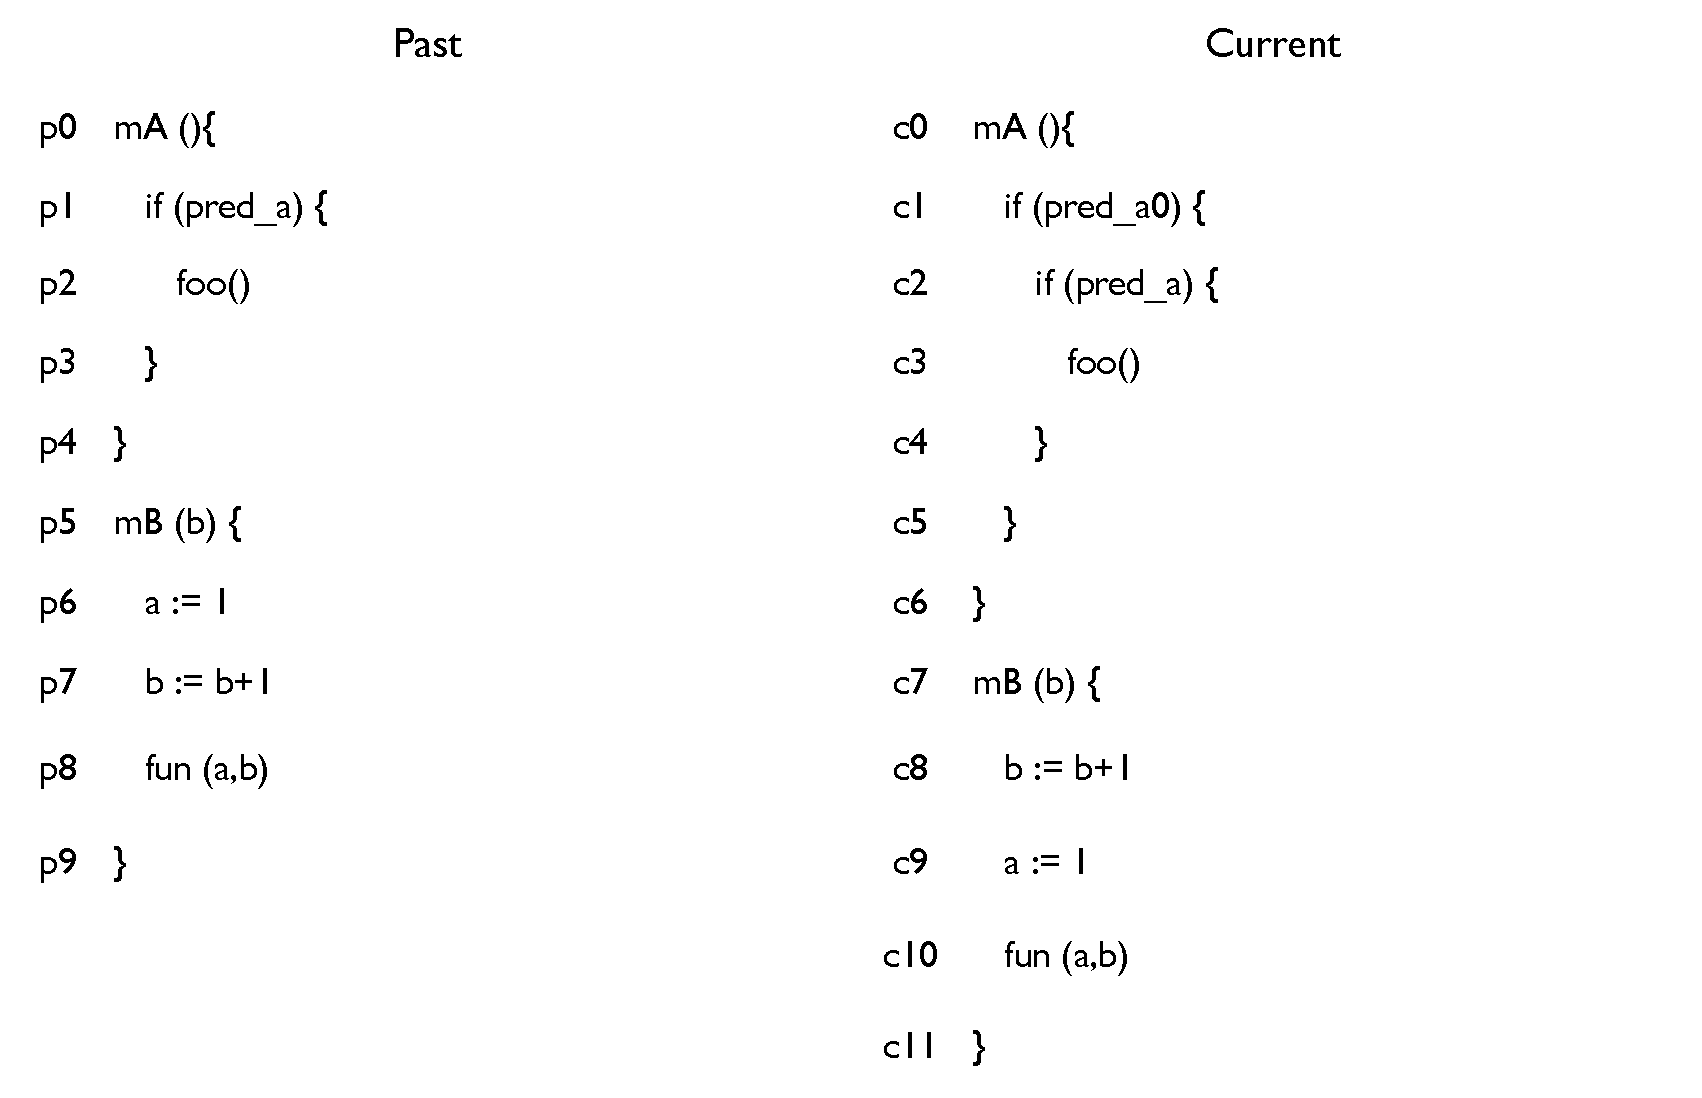
\includegraphics[width=0.95\textwidth]{images/DifferencingExample.pdf}
\caption{Example code change}
\label{fig:changeexample} 
\end{figure*}

Matching code across program versions poses several challenges. First, previous studies indicate that programmers often disagree about the origin of code elements; low inter-rater agreement suggests that there may be no ground truth in code matching~\cite{SKim2005}. Second, renaming, merging, and splitting of code elements that are discussed in the context of refactoring reconstruction in Section~\ref{sec:refactoringreview} make the matching problem non-trivial. Suppose that a file \codefont{PElmtMatch} changed its name to \codefont{PMatching}; a procedure \codefont{matchBlck} is split into two procedures \codefont{matchDBlck} and \codefont{matchCBlck}; and a procedure \codefont{matchAST} changed its name to \codefont{matchAbstractSyntaxTree}. The intuitively correct matching technique should produce [(\codefont{PElmtMatch, PMatching}), (\codefont{matchBlck, matchDBlck}), (\codefont{matchBlck, matchCBlck}), \\and (\codefont{matchAST, matchAbstractSyntaxTree})], while simple name-based matching will consider \codefont{PMatching}, \codefont{matchDBlck}, \codefont{matchCBlck}, and \codefont{matchAbstractSyntaxTree} added and consider \codefont{PElmtMatch}, \codefont{matchBlck}, and \codefont{matchAST} deleted.

Existing code matching techniques usually employ syntactic and textual similarity measures to match code. They can be characterized by the choices of (1) an underlying program representation, (2) matching granularity, (3) matching multiplicity, and (4) matching heuristics. Below, we categorize program differencing techniques with respect to internal program representations, and we discuss seminal papers for each representation.

\subsubsection{String and Lexical Matching.}
When a program is represented as a string, the best match between two strings is computed by finding the longest common subsequence (LCS) \cite{Apostolico1997}. The LCS problem is built on the assumption that (1) available operations are addition and deletion, and (2) matched pairs cannot cross one another. Thus, the longest common subsequence does not necessarily include all possible matches when available edit operations include copy, paste, and move. Tichy's \textit{bdiff} \cite{Tichy1984} extended the LCS problem by relaxing the two assumptions above: permitting crossing block moves and not requiring one-to-one correspondence. 


The line-level LCS implementation, \textit{diff} \cite{Hunt1977:LCS} is fast, reliable, and readily available. Thus, it has served as a basis for popular version control systems such as CVS. Many evolution analyses are based on {\it diff} because they use version control system data as input. For example, identification of fix-inducing code snippets is based on line tracking \textit{(file name:: function name:: line number)} backward from the moment that a bug is fixed~\cite{Sliwerski:2005} 

The longest common subsequence algorithm is a dynamic programming algorithm with $O(mn)$ in time and space, when $m$ is the line size of the past program and the $n$ is the line size of the current program. The goal of LCS-based diff is to report the minimum number of line changes necessary to convert one file to another. It consists of two phases: (1) computing the length of LCS and (2) reading out the longest common subsequence using a backtrace algorithm. 
%Figure~\ref{fig:lcs} shows the pseudo code and the two dimensional array used to compute the LCS. Blue boxes mean the cells where the lines are identical. The red boxes represents the back trace of reading out the LCS, which produces the 
Applying LCS to the example in Figure~\ref{fig:changeexample} will produce the line matching of [(p0-c0), (p1-c1), (p2-c3), (p3-c5), (p4-c6), (p5-c7), (p6-c9), (p8-c10), (p9-c11)]. Due to the assumption of no crossing matches, LCS does not find (p7-c8). In addition, because the matching is done at the line level and LCS does not consider the syntactic structure of code, it produces a line-level match such as (p3-c5) that do not observe the matching block parentheses rule. 

%\begin{figure*}
%\centering
%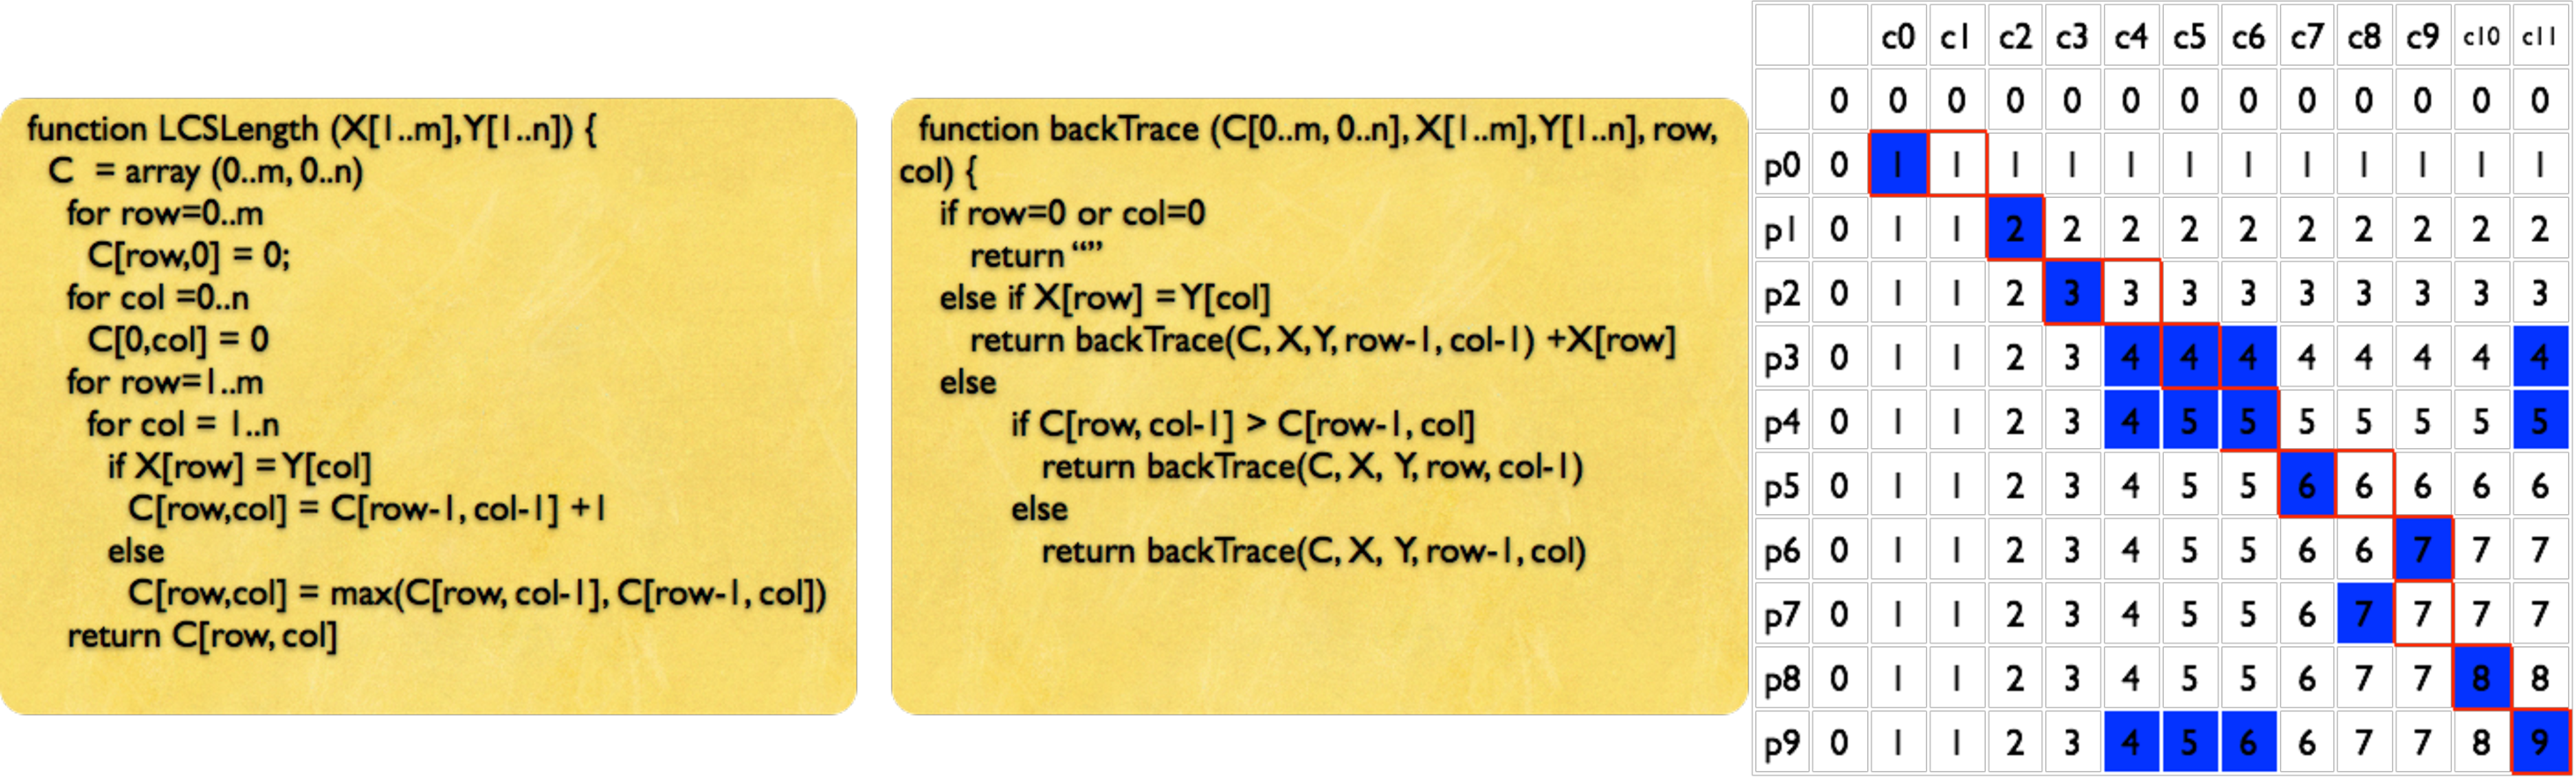
\includegraphics[width=0.95\textwidth]{images/LCS.pdf}
%\caption{Longest common subsequence (LCS) algorithm and program differencing results based on LCS}
%\label{fig:lcs} 
%\end{figure*}

%Reiss \cite{Reiss2008} evaluated practical LCS-based source line tracking techniques. His investigation shows that the {\it W\_BEST\_LINE} method\textemdash  a variation of LCS algorithm that considers $k$ number of contextual lines\textemdash is about as effective as any other method but is faster and requires only a small amount of storage. This method compares each line to derive a normalized match value between zero (no match) and one (exact match); looks at a context consisting of $k/2$ lines before and after the line; and counts the number of these lines that match the corresponding line in the new version.  

% Canfora et al. 
%Recently, Canfora et al. \cite{Canfora2007} developed a source line technique that takes differencing results from {\it diff}-based version control systems as input and identifies changed-lines in addition to added- and deleted-lines. This technique first computes hunk similarity between every possible hunk pair using a vector space model and then computes the Levenstein distance \cite{Levenstein1966} to map source lines within the mapped hunk pairs. In contrast to {\it diff}, this approach detects changed-lines in addition to deleted- and added-lines. 

\subsubsection{Syntax Tree Matching.}
For software version merging, Yang~\cite{Yang1991} developed an AST differencing algorithm. Given a pair of functions $(f_T,f_R)$, the algorithm creates two abstract syntax trees $T$ and $R$ and attempts to match the two tree roots. Once the two roots match, the algorithm aligns $T$'s subtrees ${t_1, t_2, ..., t_i}$ and $R$'s subtrees ${r_1, r_2, ... r_j}$ using the LCS algorithm and maps subtrees recursively. This type of tree matching respects the parent-child relationship as well as the order between sibling nodes, but is very sensitive to changes in nested blocks and control structures because tree roots must be matched for every level. 
%Figure~\ref{fig:AST} shows the abstract tree representations of the code example shown in Figure~\ref{fig:changeexample}. Figure~\ref{fig:YangDiff} shows its AST differencing algorithm in pseudo-code and the differencing results.  
Because the algorithm respects parent-child relationships when matching code, all matches are observe the syntactic boundary of code and  the matching block parentheses rule. Similar to LCS, because Yang's algorithm aligns subtrees at the current level by LCS, it cannot find crossing matches caused by code reordering. Furthermore, the algorithm is very sensitive to tree level changes or insertion of new control structures in the middle, because Yang's algorithm performs top-down AST matching. 

\begin{comment}
\begin{figure*}
\centering
\begin{minipage}{.45\textwidth}
  \centering
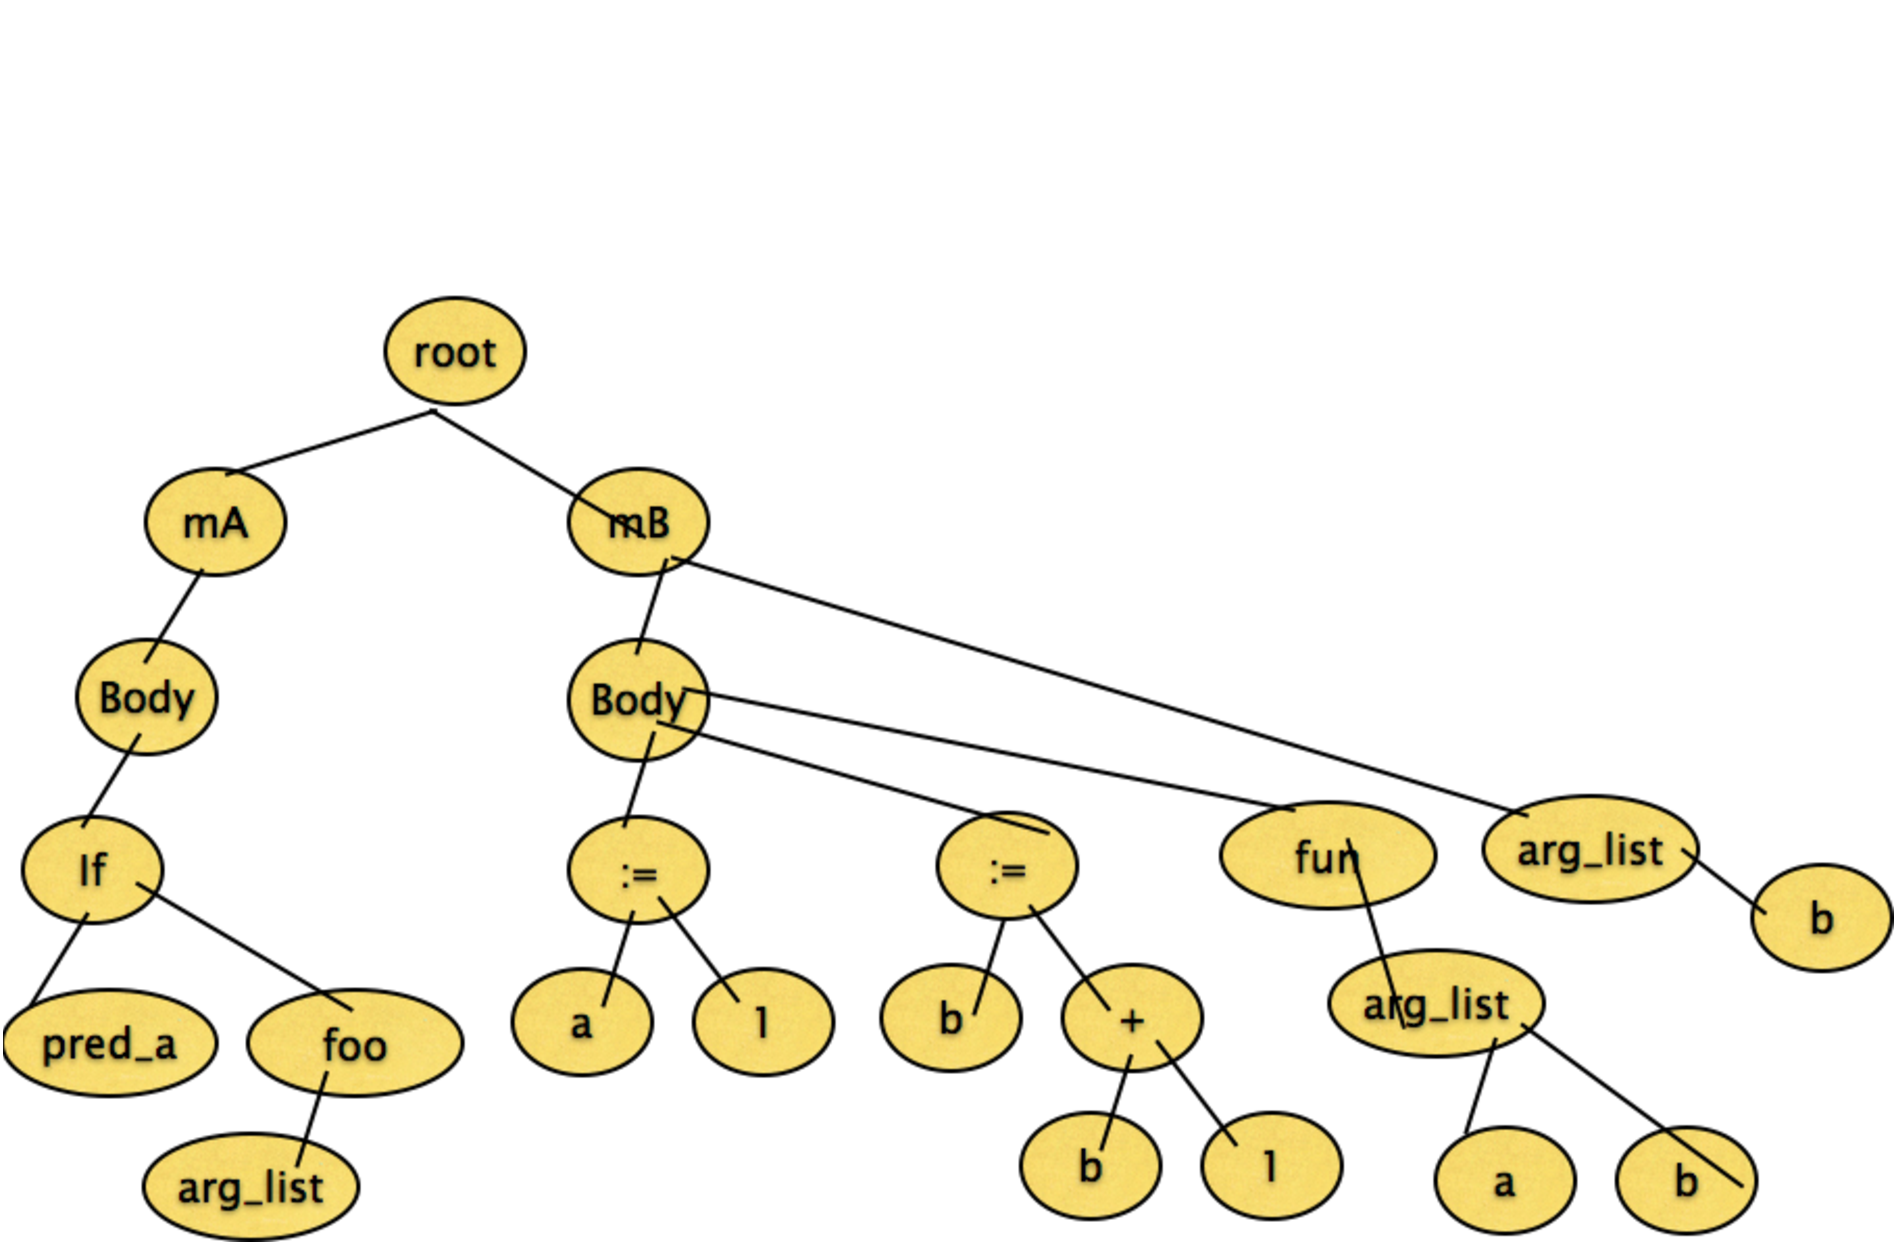
\includegraphics[width=0.9\textwidth]{images/PastAST.pdf}
\end{minipage}
\begin{minipage}{.45\textwidth}
  \centering
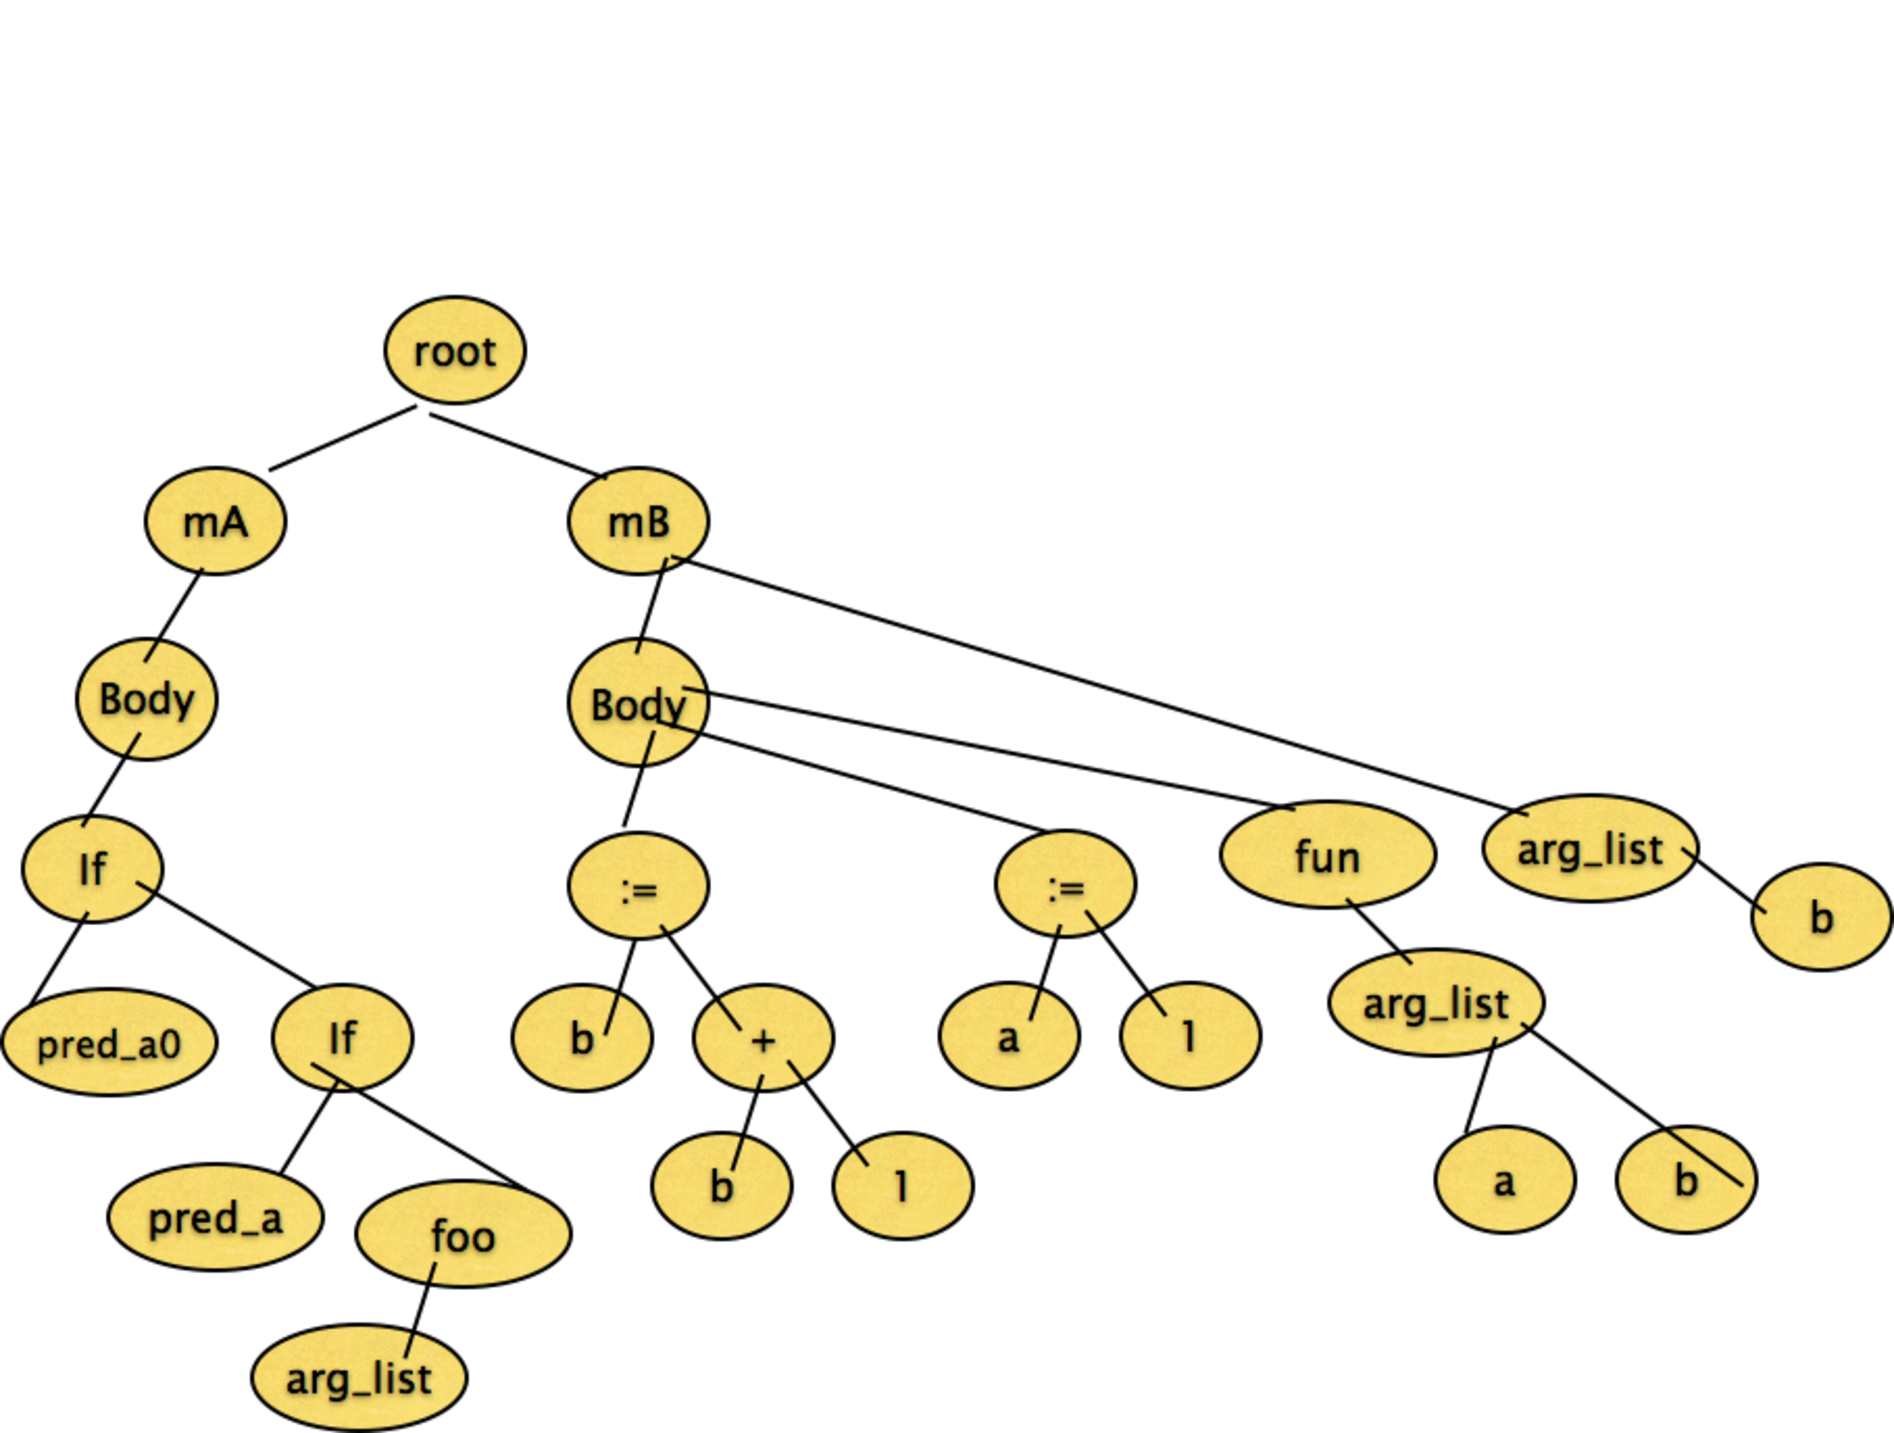
\includegraphics[width=0.9\textwidth]{images/CurrentAST.pdf}
\end{minipage}
\caption{Abstract Syntax Tree: Past (left) and Current (right)} 
\label{fig:AST} 
\end{figure*}

\begin{figure*}
\centering
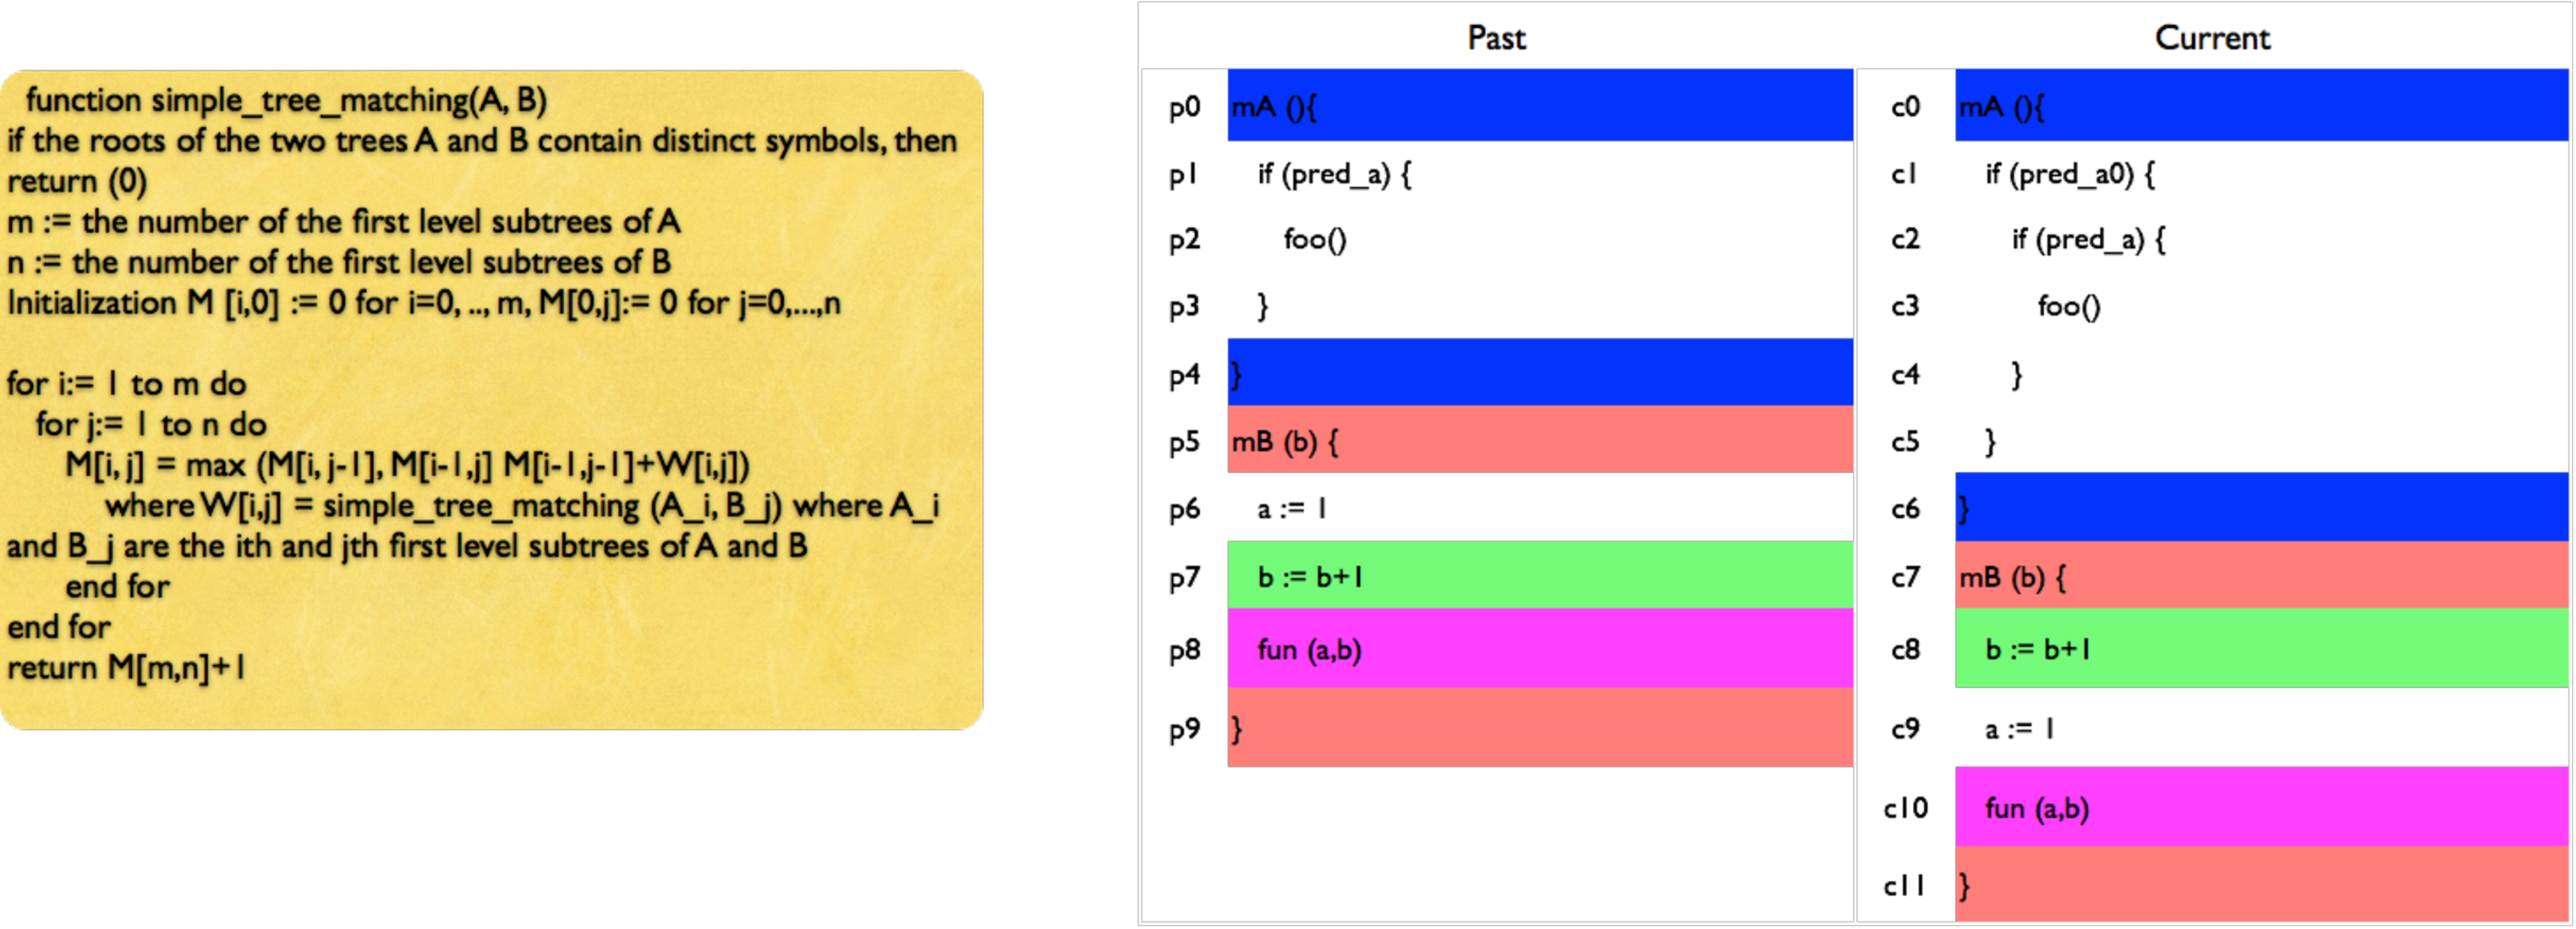
\includegraphics[width=0.95\textwidth]{images/Yang.pdf}
\caption{Yang's Abstract Syntax Tree differencing algorithm and results} 
\label{fig:YangDiff} 
\end{figure*}
\end{comment} 

%For dynamic software updating, Neamtiu et al. \cite{Neamtiu2005} built an AST-based algorithm that tracks simple changes to variables, types, and functions. Neamtiu's algorithm assumes that function names are relatively stable over time.  It traverses two ASTs in parallel; matches the ASTs of functions with the same name; and incrementally adds one-to-one mappings as long as the ASTs have the same shape. In contrast to Yang's algorithm, it cannot compare structurally different ASTs. 

% Change Distiller 
As another example, Change Distiller~\cite{FWP2007} uses an improved version of Chawathe et al.'s hierarchically structured data comparison algorithm \cite{Chawathe1996}. Change Distiller takes two abstract syntax trees as input and computes basic tree edit operations such as {\it insert, delete, move} or {\it update} of tree nodes. It uses {\it bi-gram string similarity} to match source code statements such as method invocations and uses {\it subtree similarity} to match source code structures such as if-statements. After identifying tree edit operations, Change Distiller maps each tree-edit to an atomic AST-level change type. 

% R. Walker Cottrell et al.'s Breakaway \cite{Cottrell:2007} automatically identifies detailed structural correspondences between two abstract syntax trees to help programmers generalize two pieces of similar code. Its two-pass greedy algorithm is applied to ordered child list properties (statements in a block) then to unordered nodes (method declarations). 

% Finally, the following two techniques do not directly compare ASTs but use syntactic information to guide string level differencing.  Hunt and Tichy's 3-way merging tool \cite{Hunt2002} parses a program into a language neutral form; compares token strings using the LCS algorithm; and finds syntactic changes using structural information from the parse. Raghavan et al.'s Dex \cite{Raghavan:2004:Dex} locates the changed parts in C source code files using {\it patch} file information and feeds the changed parts into a tree differencing algorithm to output the edit operations. 

\subsubsection{Control Flow Graph Matching.}
Laski and Szermer \cite{Laski1992} first developed an algorithm that computes one-to-one correspondences between CFG nodes in two programs. This algorithm reduces a CFG to a series of single-entry, single-exit subgraphs called hammocks and matches a sequence of hammock nodes using a depth first search (DFS). Once a pair of corresponding hammock nodes is found, the hammock nodes are recursively expanded in order to find correspondences within the matched hammocks. 
 
\textit{Jdiff} \cite{Apiwattanapong2004} extends Laski and Szermer's (LS) algorithm to compare Java programs based on an enhanced control flow graph (ECFG). \textit{Jdiff} is similar to the LS algorithm in the sense that hammocks are recursively expanded and compared, but is different in three ways: First, while the LS algorithm compares hammock nodes by the name of a start node in the hammock, \textit{Jdiff} checks whether the ratio of unchanged-matched pairs in the hammock is greater than a chosen threshold in order to allow for flexible matches. Second, while the LS algorithm uses DFS to match hammock nodes, \textit{Jdiff} only uses DFS up to a certain look-ahead depth to improve its performance. Third, while the LS algorithm requires hammock node matches at the same nested level, \textit{Jdiff} can match hammock nodes at a different nested level; thus, \textit{Jdiff} is more robust to addition of while loops or if-statements at the beginning of a code segment. \textit{Jdiff} has been used for regression test selection \cite{Orso2004} and dynamic change impact analysis \cite{Apiwattanapong2005}. Figure~\ref{fig:JDiff} shows the code example and corresponding extended control flow graph representations in Java. Because their representation and matching algorithm is designed to account for dynamic dispatching and exception handling, it can detect changes in the method body of \codefont{m3 (A a)}, even though it did not have any textual edits: (1) \codefont{a.m1()} calls the method definition \codefont{B.m()} for the receiver object of type B and (2) when the exception type \codefont{E3} is thrown, it is caught by the catch block \codefont{E1} instead of the catch block \codefont{E2}.   

\begin{figure*}
\centering
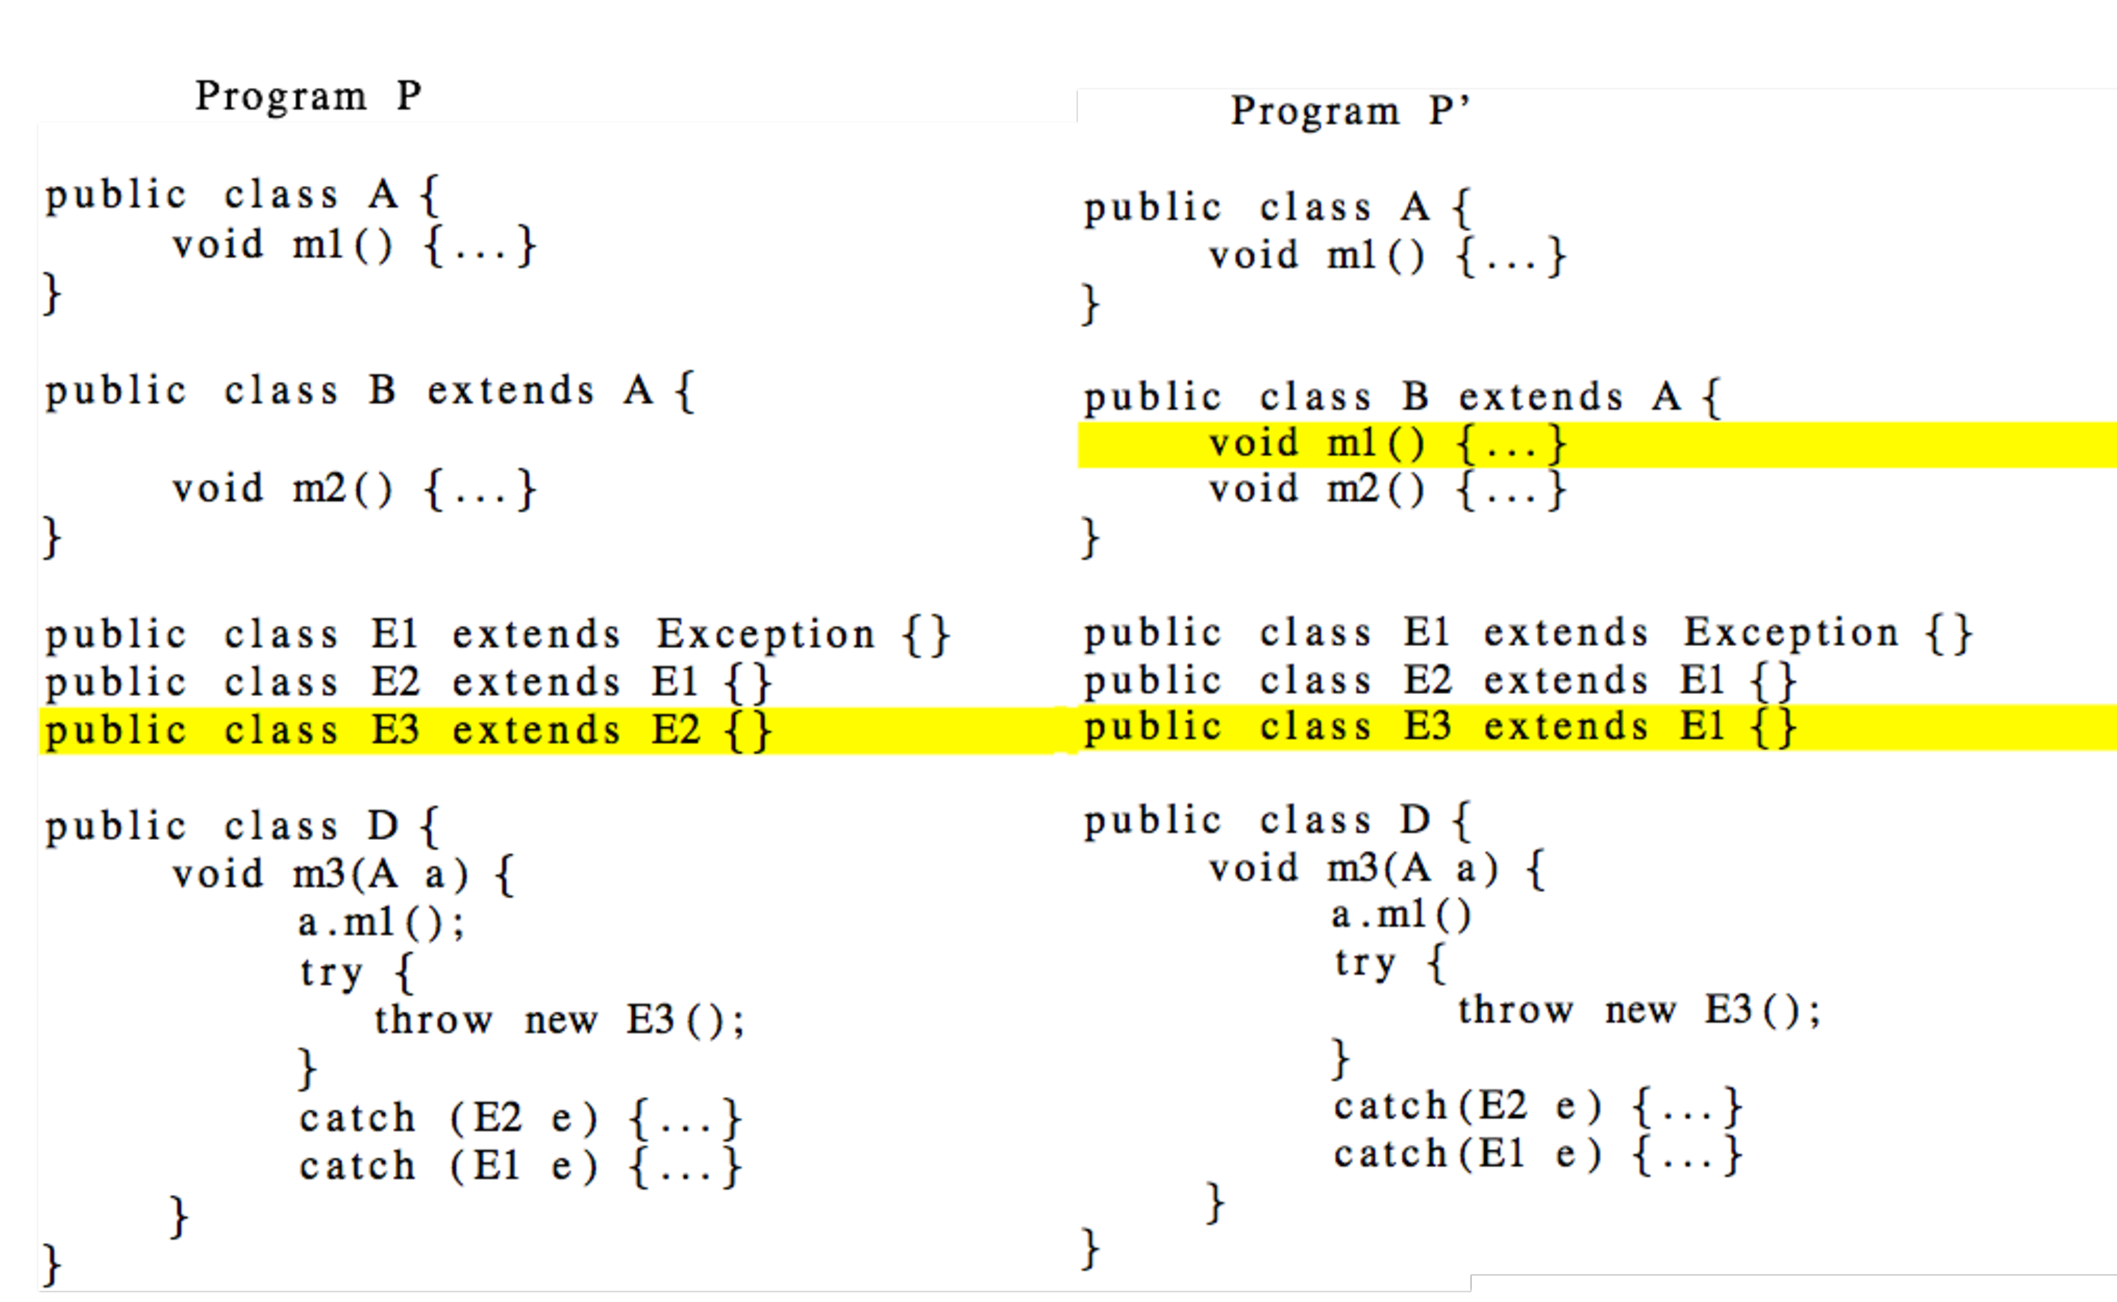
\includegraphics[width=0.95\textwidth]{images/JDiffCodeExample.pdf}
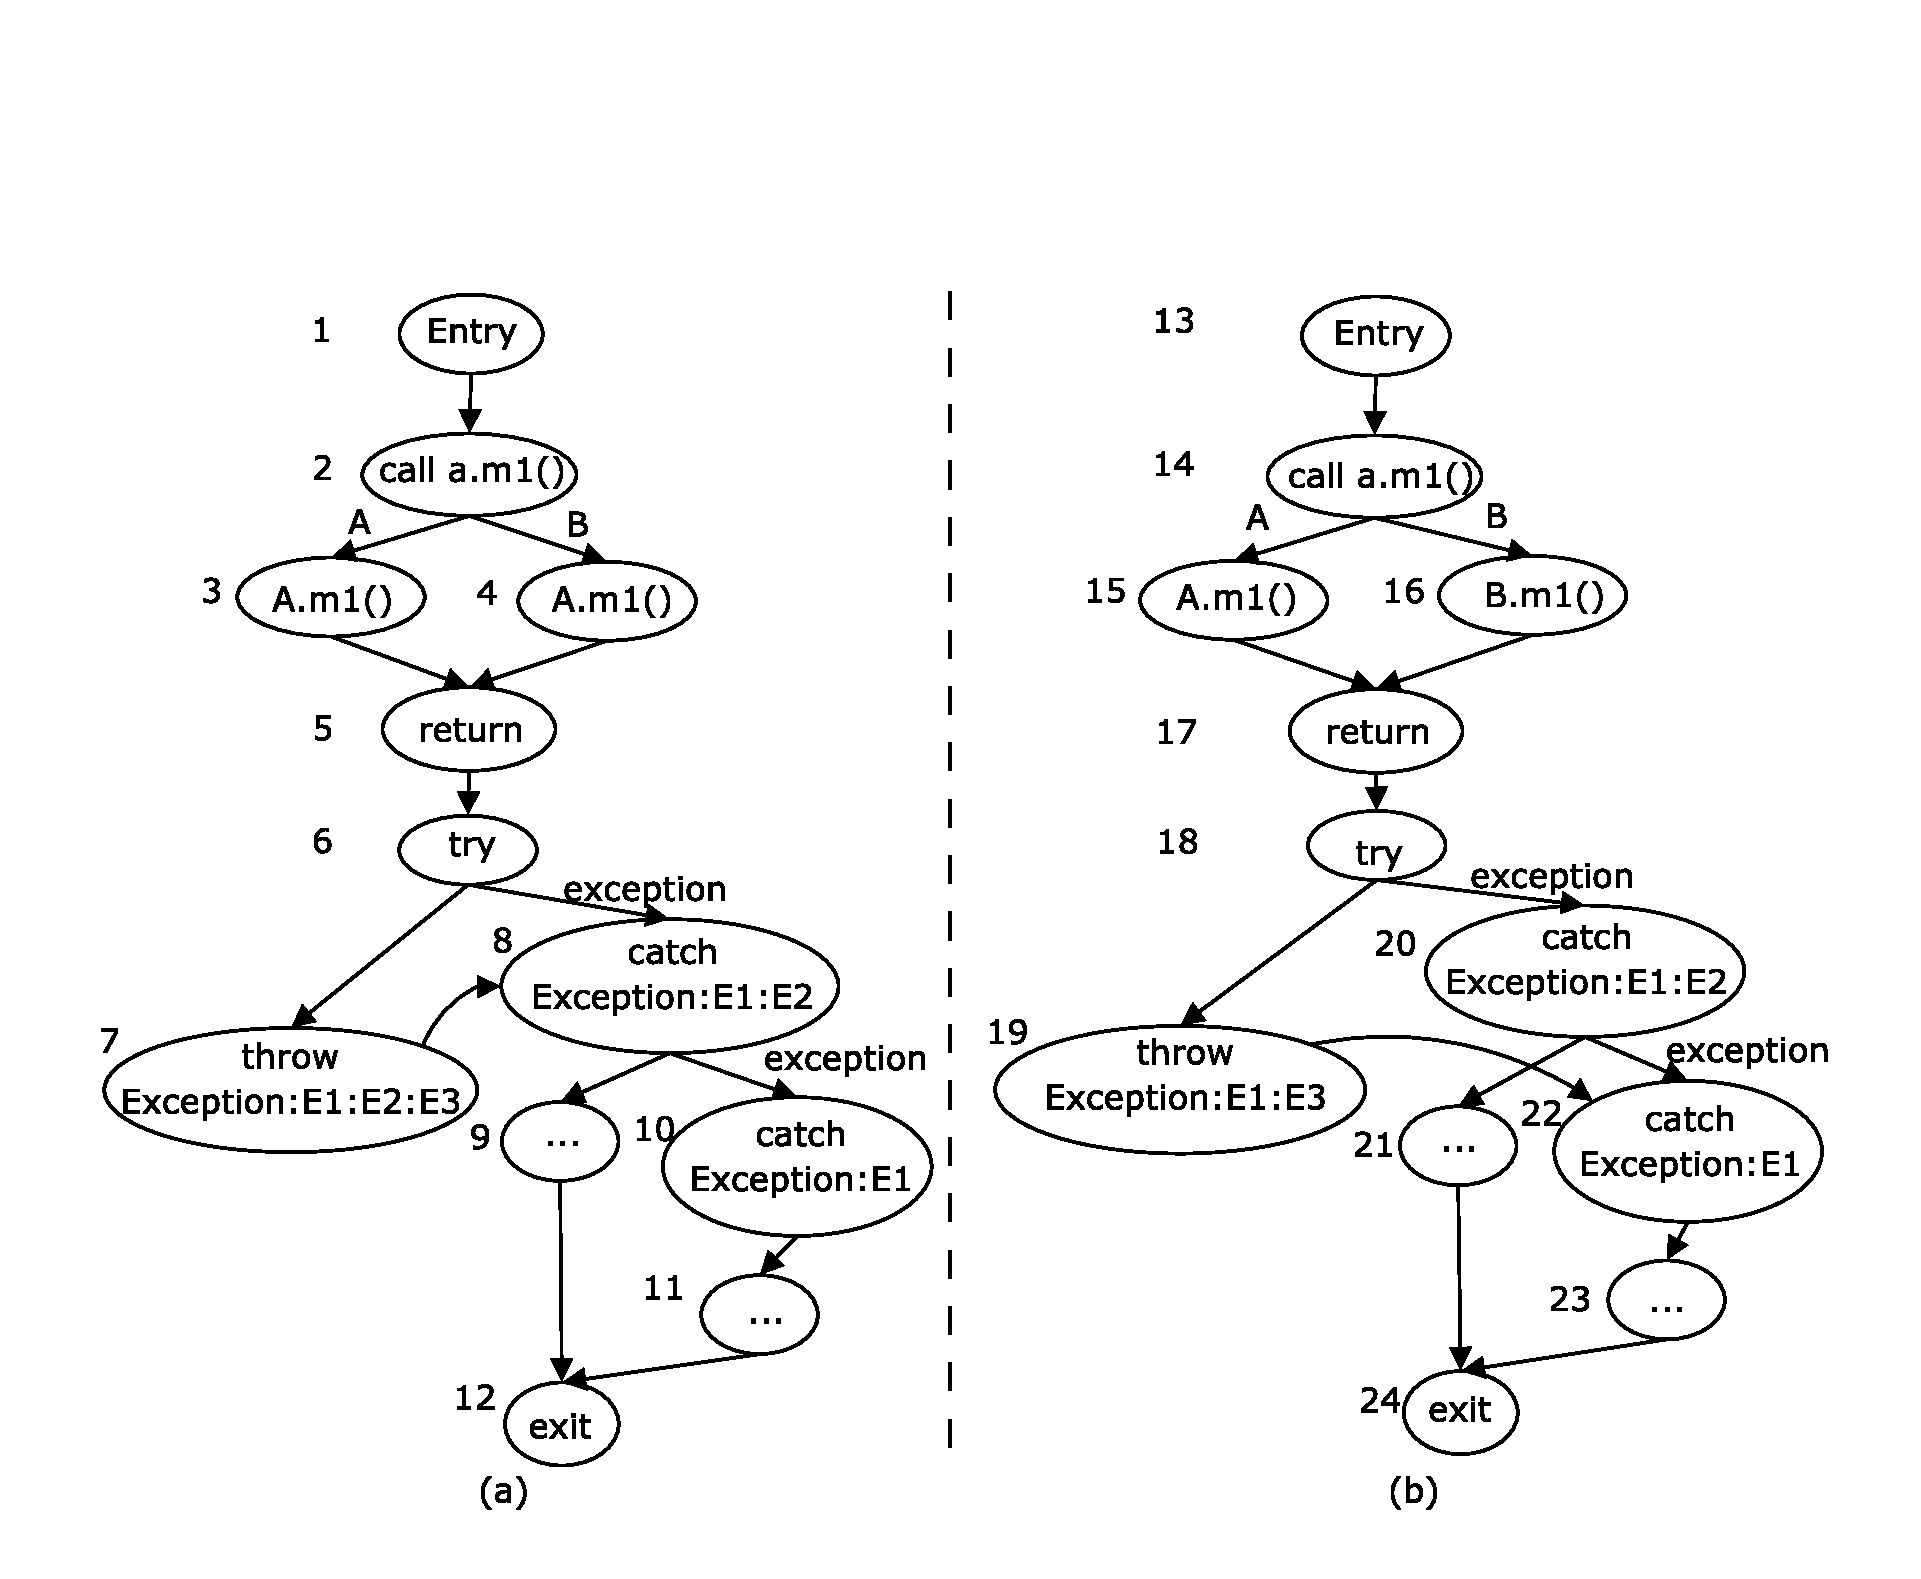
\includegraphics[width=0.95\textwidth]{images/JDiffCFG.pdf}
\caption{JDiff Change Example and CFG representations~\cite{Apiwattanapong2005}} 
\label{fig:JDiff} 
\end{figure*}

CFG-like representations are commonly used in regression test selection research. Rothermel and Harrold \cite{Rothermel1997} traverse two CFGs in parallel and identify a node with unmatched edges, which indicates changes in code. In other words, their algorithm stops parallel traversal as soon as it detects changes in a graph structure; thus, this algorithm does not produce deep structural matches between CFGs. However, traversing graphs in parallel is still sufficient for the regression testing problem because it conservatively identifies affected test cases. In practice, regression test selection algorithms~\cite{Harrold2001, Orso2004} require that syntactically changed classes and interfaces are given as input to the CFG matching algorithm. 

\subsubsection{Program Dependence Graph Matching.}
There are several program differencing algorithms based on a program dependence graph \cite{Horwitz1990, Binkley1995, Jackson1994}. 

Horwitz \cite{Horwitz1990} presents a semantic differencing algorithm that operates on a program representation graph (PRG) which combines features of program dependence graphs and static single assignment forms. In her definition, semantic equivalence between two programs $P1$ and $P2$ means that, for all states $\sigma$ such that $P1$ and $P2$ halt, the sequence of values produced at $c1$ is identical to the sequence of values produced at $c2$ where $c1$ and $c2$ are corresponding locations. 
Horwitz uses Yang's algorithm \cite{Yang1989} to partition the vertices into a group of semantically equivalent vertices based on three properties, (1) the equivalence of their operators, (2) the equivalence of their inputs, (3) the equivalence of the predicates controlling their evaluation. The partitioning algorithm starts with an initial partition based on the operators used in the vertices. Then by following flow dependence edges, it refines the initial partition if the successors of the same group are not in the same group. Similarly, it further refines the partition by following control dependence edges. If two vertices in the same partition are textually different, they are considered to have only a {\it textual change}. If two vertices are in different partitions, they have a {\it semantic change}. After the partitioning phase, the algorithm finds correspondences between $P1$'s vertices and $P2$'s vertices that minimize the number of semantically or textually changed components of $P2$. 
% semantic change: no matching partition. 
% textual change: same partition but different text. 
% same: same partition and same text. 
In general, PDG-based algorithms are not applicable to popular modern program languages because they can run only on a limited subset of C-like languages without global variables, pointers, arrays, or procedures. 

%Binkley et al. \cite{Binkley1995} presents a 3-way merging algorithm that is based on semantic differences. This algorithm does not find corresponding elements between two versions of a program, but rather makes an assumption that a special editor is used to tag each PDG node to identify added nodes, deleted nodes and changed nodes. Given PDG node level correspondence among three input programs A, B, and Base, the integration algorithm produces a program M that integrates the difference A from Base, the difference B from Base, and the preserved behavior among A, B, and Base. The behavior differences between A and B are approximated by the slice of $AP_{A,Base}$ in $G_A$ where $AP_{A,Base}$ is a set of vertices of $G_A$ whose program slice is different from $G_{Base}$'s slice. Although the problem of determining  whether $G_M$ corresponds to some program is NP-complete, Binkley et al. presented a backtracking algorithm that behaves satisfactorily on actual programs. 

\subsubsection{Related Topics: Model Differencing and Clone Detection.} 

A clone detector is simply an implementation of an arbitrary equivalence function. The equivalence function defined by each clone detector depends on a program representation and a comparison algorithm. Most clone detectors are heavily dependent on (1) hash functions to improve performance, (2) parametrization to allow flexible matches, and (3) thresholds to remove spurious matches. A clone detector can be considered as a many-to-many matcher based solely on content similarity heuristics. 

In addition to these, several differencing algorithms compare model elements~\cite{UMLDiff2005, Ohst2003:umldiff, Soto2006:deltaprocess, Duley2012:vdiff}. For example, UMLdiff~\cite{UMLDiff2005} matches methods and classes between two program versions based on their name. However, these techniques assume that no code elements share the same name in a program and thus use name similarity to produce one-to-one code element matches. Some have developed a general, meta-model based, configurable program differencing framework~\cite{Schmidt2008:sidiff, EMF}. For example, SiDiff \cite{Schmidt2008:sidiff,Treude2007} allows tool developers to configure various matching algorithms such as identity-based matching, structure-based matching, and signature-based matching by defining how different types of elements need to be compared and by defining the weights for computing an overall similarity measure.


